%% marl_multi, algorithm -> PHY: one box per file, call flow top to bottom,
%% the PHY sealed (no internals). File names are the tags above each box,
%% anchored to the boxes so they can never drift into them.
\documentclass[tikz,border=5pt]{standalone}
\usepackage{xcolor}
%% Shared look for the UnionLabs system figures. \input by each fig-*.tex so a
%% colour or a corner radius is changed in one place.
\usetikzlibrary{positioning,arrows.meta,fit,backgrounds,calc}

\definecolor{uCode}{HTML}{1F6F5C}     % the experimenter's own code
\definecolor{uApi}{HTML}{6B4BA8}      % the contract / ARQ layer
\definecolor{uPhy}{HTML}{2E5E9E}      % transports / DSP
\definecolor{uRadio}{HTML}{B4700F}    % hardware
\definecolor{uShare}{HTML}{8A2E4D}    % the shared workspace

\tikzset{
  blk/.style={draw, rounded corners=2pt, align=center, font=\small,
              minimum height=8mm, inner sep=3pt, fill=black!2},
  code/.style={blk, draw=uCode, thick, fill=uCode!6},
  api/.style={blk, draw=uApi, very thick, fill=uApi!7},
  phy/.style={blk, draw=uPhy, thick, fill=uPhy!6},
  radio/.style={blk, draw=uRadio, thick, fill=uRadio!8},
  share/.style={blk, draw=uShare, thick, fill=uShare!6},
  stage/.style={blk, minimum height=9.5mm, font=\scriptsize, text width=16mm,
                inner sep=2pt},
  flow/.style={-{Latex[length=2mm]}, thick},
  back/.style={-{Latex[length=2mm]}, thick, densely dashed},
  % labels that sit ON an arrow: opaque, so the line never strikes the text
  onarrow/.style={font=\scriptsize\itshape, fill=white, inner sep=1.5pt},
  lbl/.style={font=\scriptsize\itshape, inner sep=1pt},
  note/.style={font=\scriptsize, align=left, inner sep=1pt},
  legend/.style={draw, minimum width=3mm, minimum height=3mm, inner sep=0pt},
}
\newcommand{\mono}[1]{{\ttfamily\footnotesize #1}}
\newcommand{\monos}[1]{{\ttfamily\scriptsize #1}}

\begin{document}
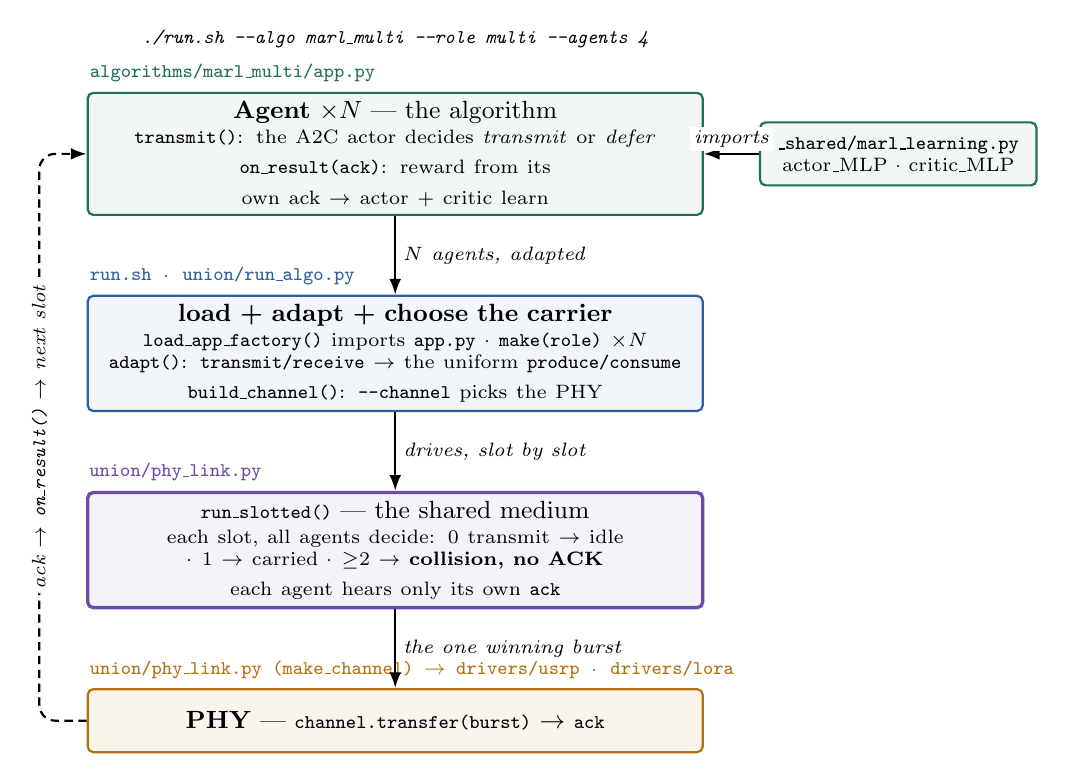
\begin{tikzpicture}[x=1mm, y=1mm,
  b/.style={blk, text width=76mm, font=\small, align=center},
  tag/.style={font=\ttfamily\scriptsize\bfseries, inner sep=1pt, anchor=south west}]

\node[lbl, anchor=south, align=center] at (0,13)
  {\monos{./run.sh --algo marl\_multi --role multi --agents 4}};

%% ── the algorithm ─────────────────────────────────────────────────────────
\node[b, code] (app) at (0,0)
  {\textbf{Agent} $\times N$ --- the algorithm\\[1pt]
   {\scriptsize \monos{transmit()}: the A2C actor decides
    \emph{transmit} or \emph{defer}\\
    \monos{on\_result(ack)}: reward from its own ack
    $\rightarrow$ actor + critic learn}};
\node[tag, text=uCode] at ([yshift=0.8mm]app.north west)
  {algorithms/marl\_multi/app.py};

\node[b, code, text width=33mm, right=7mm of app, font=\scriptsize] (nets)
  {\monos{\_shared/marl\_learning.py}\\actor\_MLP · critic\_MLP};
\draw[flow] (nets) -- node[onarrow, above=0.5pt] {imports} (app);

%% ── the middleware ────────────────────────────────────────────────────────
\node[b, phy, below=10mm of app] (ra)
  {\textbf{load + adapt + choose the carrier}\\[1pt]
   {\scriptsize \monos{load\_app\_factory()} imports \monos{app.py} ·
    \monos{make(role)} $\times N$\\
    \monos{adapt()}: \monos{transmit/receive} $\rightarrow$ the uniform
    \monos{produce/consume}\\
    \monos{build\_channel()}: \monos{--channel} picks the PHY}};
\node[tag, text=uPhy] at ([yshift=0.8mm]ra.north west)
  {run.sh · union/run\_algo.py};

%% ── the runner ────────────────────────────────────────────────────────────
\node[b, api, below=10mm of ra] (loop)
  {\textbf{\monos{run\_slotted()}} --- the shared medium\\[1pt]
   {\scriptsize each slot, all agents decide: 0 transmit $\rightarrow$ idle ·
    1 $\rightarrow$ carried · $\geq$2 $\rightarrow$ \textbf{collision, no ACK}\\
    each agent hears only its own \monos{ack}}};
\node[tag, text=uApi] at ([yshift=0.8mm]loop.north west)
  {union/phy\_link.py};

%% ── the PHY, sealed ───────────────────────────────────────────────────────
\node[b, radio, below=10mm of loop] (phy)
  {\textbf{PHY} --- \monos{channel.transfer(burst)} $\rightarrow$ \monos{ack}};
\node[tag, text=uRadio] at ([yshift=0.8mm]phy.north west)
  {union/phy\_link.py (\mbox{make\_channel}) $\rightarrow$ drivers/usrp · drivers/lora};

%% ── flow ──────────────────────────────────────────────────────────────────
\draw[flow] (app) -- node[onarrow, right=1pt] {$N$ agents, adapted} (ra);
\draw[flow] (ra) -- node[onarrow, right=1pt] {drives, slot by slot} (loop);
\draw[flow] (loop) -- node[onarrow, right=1pt] {the one winning burst} (phy);
\draw[back, rounded corners=2mm]
  (phy.west) -- ++(-6,0) |-
  node[pos=0.25, onarrow, rotate=90]
  {ack $\rightarrow$ \monos{on\_result()} $\rightarrow$ next slot}
  (app.west);

\end{tikzpicture}
\end{document}
